\documentclass{article}

% if you need to pass options to natbib, use, e.g.:
% \PassOptionsToPackage{numbers, compress}{natbib}
% before loading nips_2018

% ready for submission
\usepackage{nips_2018}

% to compile a preprint version, e.g., for submission to arXiv, add
% add the [preprint] option:
% \usepackage[preprint]{nips_2018}

% to compile a camera-ready version, add the [final] option, e.g.:
% \usepackage[final]{nips_2018}

% to avoid loading the natbib package, add option nonatbib:
% \usepackage[nonatbib]{nips_2018}

\usepackage[utf8]{inputenc} % allow utf-8 input
\usepackage[T1]{fontenc}    % use 8-bit T1 fonts
\usepackage{hyperref}       % hyperlinks
\usepackage{url}            % simple URL typesetting
\usepackage{booktabs}       % professional-quality tables
\usepackage{amsfonts}       % blackboard math symbols
\usepackage{amsmath}
\usepackage{amssymb}
\usepackage{nicefrac}       % compact symbols for 1/2, etc.
\usepackage{microtype}      % microtypography
\usepackage{algorithm}
\usepackage{graphicx}
%\usepackage{subfig}
\usepackage{subcaption}
\usepackage{color}
\usepackage{bm}

\usepackage{amsmath}
\usepackage[noend]{algpseudocode}

\title{Target Encoding Networks}

% The \author macro works with any number of authors. There are two
% commands used to separate the names and addresses of multiple
% authors: \And and \AND.
%
% Using \And between authors leaves it to LaTeX to determine where to
% break the lines. Using \AND forces a line break at that point. So,
% if LaTeX puts 3 of 4 authors names on the first line, and the last
% on the second line, try using \AND instead of \And before the third
% author name.

\author{
  David S.~Hippocampus\thanks{Use footnote for providing further
    information about author (webpage, alternative
    address)---\emph{not} for acknowledging funding agencies.} \\
  Department of Computer Science\\
  Cranberry-Lemon University\\
  Pittsburgh, PA 15213 \\
  \texttt{hippo@cs.cranberry-lemon.edu} \\
  %% examples of more authors
  %% \And
  %% Coauthor \\
  %% Affiliation \\
  %% Address \\
  %% \texttt{email} \\
  %% \AND
  %% Coauthor \\
  %% Affiliation \\
  %% Address \\
  %% \texttt{email} \\
  %% \And
  %% Coauthor \\
  %% Affiliation \\
  %% Address \\
  %% \texttt{email} \\
  %% \And
  %% Coauthor \\
  %% Affiliation \\
  %% Address \\
  %% \texttt{email} \\
}

\begin{document}
% \nipsfinalcopy is no longer used

\maketitle

\begin{abstract}
  We consider the problem of prediction in a highly uncertain environment.
\end{abstract}


\section{Introduction}

Learning to predict future states of a complex time series, such as sensory inputs, is an important research problem with applications in unsupervised learning, planning, and compression.
A significant difficulty is the inherently uncertain nature of many such time series: for example, given an initial part of a video sequence, there are often many ways in which the rest of the sequence can unfold.
The space of possible futures can form a set of discrete modes, a connected manifold, or some combination of these, and training with classical $\ell_1$ or $\ell_2$ losses will predict the median or the mean of the set of possible futures, which often does not itself constitute a valid prediction.

One approach is to learn the parameters of a distribution over the set of possible future states, for example a Gaussian Mixture Model \citep{mixture-density-networks}.
This has been successfully used when the dimensionality is low, but is not practical when the states are high-dimensional.
More recently, several works have been proposed which use the framework of conditional Variational AutoEncoders (VAEs) for generating images and video frames.
VAEs assume a prior over latent variables and include a loss term measuring the Kullback–Leibler (KL) divergence between this prior and the distribution output by the posterior network.
This helps ensure that latent variables sampled from this prior at generation time are consistent with those input to the decoder network during training.
Simple priors, such as diagonal Gaussians, are common choices, as they enable a closed-form expression for the KL divergence between prior and posterior distributions, which in turn reduces the variance of the gradients with respect to this term.
One issue with VAEs is the so-called ``posterior collapse'' or ``over-regularization'' problem, which is caused by a conflict between the prior matching term and the reconstruction term in the loss function. If the regularization term is too high, this can cause the model to ignore the latent variables altogether in order to avoid a high cost due to the KL term. If the regularization term is too low, this can cause the model to learn a latent variable distribution which does not match with the assumed prior, leading to poor generations at test time.
Therefore, careful tuning of the prior term, or annealing schedules, are often required.

In this work, we propose an alternate approach which does not place any priors on the latent variable distribution and instead relies on a non-parametric or semi-parametric sampling procedure to produce new generations at test time.
It is simple to implement, contains a single term in the loss function, and does not run the risk of mode collapse.
By removing the prior assumption, we also do away with the need for a regularization term at training time, which enforces a match between prior and posterior distributions, leading to a simple and easy-to-optimize loss.
After training, we obtain a non-parametric estimate of the distribution over latent variables by extracting a collection of latent variables from the training set itself, which we then combine with new inputs to obtain generations.
Through this non-parametric sampling procedure, we naturally obtain samples which are on the manifold of latent variables.
If the prior distribution over latent variables is dependent on the input, it may additionally be necessary to restrict our sampling to a limited region of the manifold.
We therefore propose and empirically investigate two ways of achieving this: (1) through a smoothness assumption on the trajectories of latent variables along the manifold, which translates into a nearest-neighbor based sampling scheme, and (2) by combining the non-parametric sampling scheme with a parametric likelihood model which restricts our sampling to a subregion of the manifold.

The contributions of this work are the following:
\begin{itemize}
\item New large-scale dataset with applications for autonomous driving
\item We introduce a novel method for prediction under uncertainty which is simple to train, does not make assumptions about a prior distribution over latent variables or require sampling at training time, and is able to generate diverse predictions many timesteps into the future.
\end{itemize}


\section{Predictive Model}

\subsection{Architecture and Training}

\begin{figure}
  \centering
  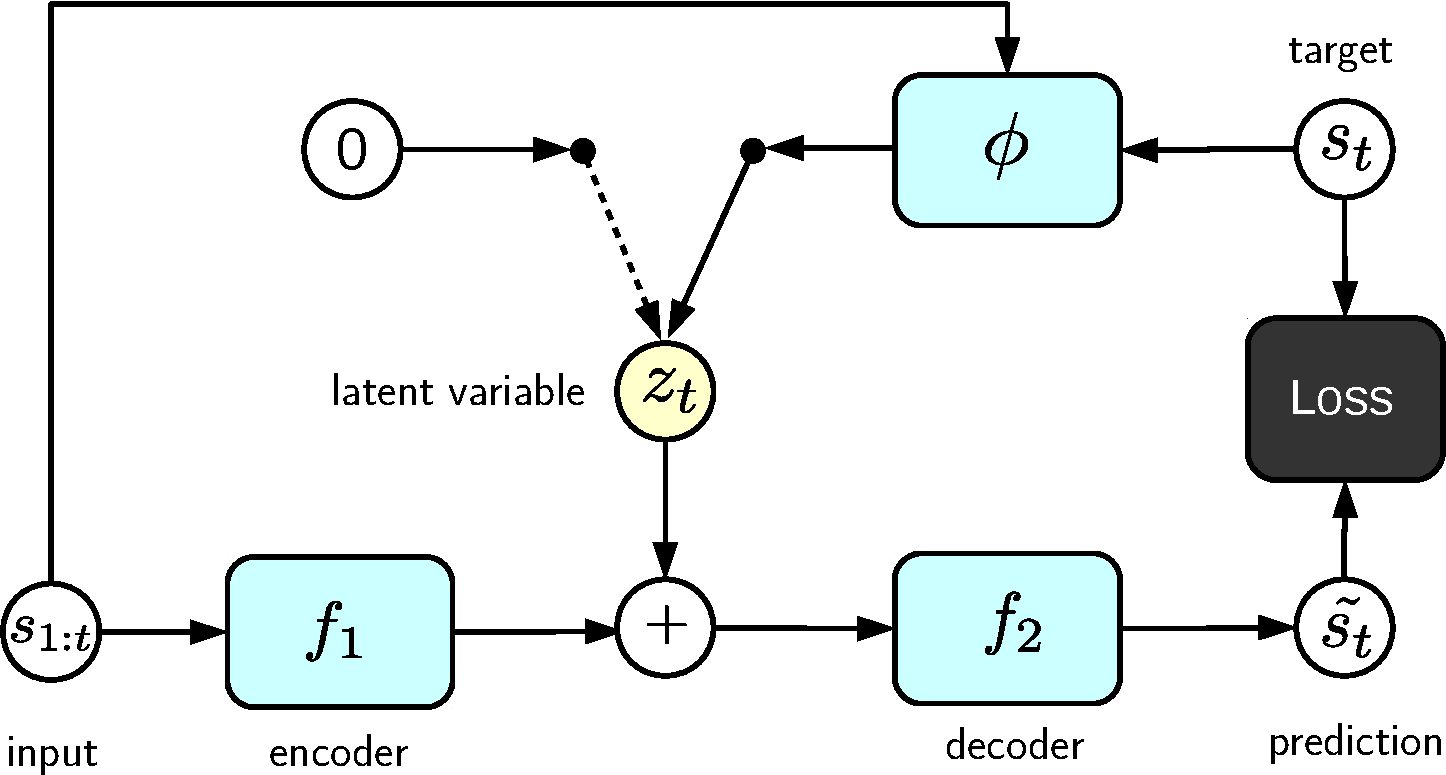
\includegraphics[width=0.5\textwidth]{images/ae_train-crop.pdf}
  \caption{Prediction Model. }
\end{figure}

Our stochastic prediction model can be viewed as a conditional autoencoder paired with a non-parametric  or semi-parametric sampling procedure.
The architecture consists of three neural networks: an encoder $f_\text{enc}$, a decoder $f_\text{dec}$ and a latent variable network $f_\phi$.
For each input $s_{1:t}$ (\emph{i.e.}\ a sequence of $t$ consecutive states) and a target $s_{t+1}$ (\emph{i.e.}\ the following state), the update equations are given by:
%
\begin{align}
  z_t &=
  \begin{cases}
    \bm{0} & \mbox{   if   } u = 1, \mbox{   } u \sim \mathcal{B}(p) \\
    f_\phi(s_{1:t}, s_{t+1}) & \mbox{   otherwise}
  \end{cases} \\
  \hat{s}_{t+1} &= f_\text{dec}(f_\text{enc}(s_{1:t}), z_t) = f_\theta(s_{1:t}, z_t)
\end{align}
%
where $z_t$ is the latent variable vector associated to the input $s_{1:t}$, $\hat{s}_{t + 1}$ is the reconstructed target state, and $\mathcal{B}(p)$ is a Bernoulli random variable with probability $p$.
All networks are trained by gradient descent to optimize the following objective:
%
\begin{align}
  \ell(\hat{s}_{t+1}, s_{t+1}) &= \lVert \hat{s}_{t+1} - s_{t+1} \rVert_2^2 \\
  &= \lVert f_\theta(s_{1:t}, z_t) - s_{t+1} \rVert_2^2
\end{align}

Note in particular that no sampling or reparamaterization is done at training time.
In standard autoencoders, some mechanism is used to limit the information content of the latent representation to avoid learning trivial mappings and thus encourage the model to learn good representations.
In the conditional case we are considering, we also need such a mechanism to prevent the network from simply reconstructing $s_{t+1}$ from $z_t$ while ignoring the input $s_{1:t}$.
This is accomplished by setting the latent vector $z_t$ to zero with some probability $p$ at every training iteration.
This setting encourages the network to continue to extract as much information as possible from the input $s_{1:t}$, rather than simply trying to reconstruct the target, and only use the true target $s_{t+1}$ to reconstruct what cannot be predicted from the input.
In our experiments, we train with $p=1$ for an initial fixed number of iterations, which corresponds to purely deterministic training, after which we reduce $p$ to incorporate the latent variables encoded from the targets.

A second key point is that the dimension of the latent variable $z_t$ is much lower than the dimension of the states $s_t$. This has two benefits: first, it can further help limit the information content and prevent trivial reconstructions of the targets. Second, it allows us to use non-parametric estimates of the distribution over latent variables using a reasonable number of points, which we detail in the next section.

%In our experiments we found setting the dimension of $z$ to be of much lower dimension than $s$ to work well, however other methods, such as adding a sparsity or contractive penalty term, could also be used.


\begin{algorithm}[t]
  \caption{Build Stochastic Model}\label{algo-train}
  \begin{algorithmic}[1]
    \State \textbf{Input} Training set $\mathcal{D}$.
    \State Initialize networks $f_\theta, f_\phi$
    \While{not converged} \Comment{Train networks}
    \State Sample a sequence $\{s_1, ..., s_t, s_{t+1}\} \sim \mathcal{D}$
    \State $z_t = f_{\phi}(s_{1:t}, s_{t+1})$
    \State $\tilde{s}_{t+1} = f_{\theta}(s_{1:t}, z_t)$
    \State $\ell(\theta, \phi) = \|s_{t+1} - \tilde{s}_{t+1} \|_2^2$
    \State $\theta \leftarrow \theta - \eta \nabla \theta$
    \State $\phi \leftarrow \phi - \eta \nabla \phi$
    \EndWhile
    \State $\mathcal{Z} \leftarrow \varnothing$     \Comment{Estimate latent distribution}
    \For{$i = 1:N_Z$}
    \State Sample a sequence $\{s_1, ..., s_t, s_{t+1}\} \sim \mathcal{D}$
    \State $z_t = f_{\phi}(s_{1:t}, s_{t+1})$
    \State $\mathcal{Z} \leftarrow \mathcal{Z} \cup \{ z_t \}$
    \EndFor
    \Return $f_\theta, \mathcal{Z}$
  \end{algorithmic}
\end{algorithm}



\subsection{Sampling}

After the model is trained, we need a sampling scheme to pair latent variables $z$ with novel input sequences $s_{1:t}$ for which we want to generate future states.
Since we do not use any prior on the latent distribution during training, we cannot assume the latent distribution follows a known parametric form which we can sample from.
Instead, we obtain a non-parametric estimate of the distribution over latent vectors by extracting a large collection of $z$ vectors from the training set, which we refer to as $\mathcal{Z}$.
We explore three sampling methods based on this estimate, which are described explicitly in Algorithm \ref{algo-sample}.

%Our sampling scheme is based on ideas from manifold learning, for which there is an extensive literature \citep{isomap, LLE, Belkin2003, TSNE}.
%These methods assume we are given a set of points $\{x_i\}$ which are assumed to lie on a low-dimensional manifold $\mathcal{M}$, and approximate the manifold by forming a graph whose vertices are $\{x_i\}$ and whose edges (which can be weighted or unweighted) depend on the Euclidean distance between them. In particular, two points are connected by an edge if they are close in Euclidean distance, as this approximates the geodesic distance along the manifold as it becomes small.
%Paths along the manifold can then be approximated by paths along the graph, and it can be shown that given a sufficiently dense sampling of points, graph distances converge to geodesic distances \citep{Bernstein2000}.

%Our sampling scheme is based on such ideas, in particular, we can treat the vectors $z$, extracted from the training set, as points sampled from the unknown latent manifold, form a graph approximation to this manifold using these points, and sample trajectories on this manifold to generate new trajectories in the original input space.

%After training, we extract all vectors $z$ from the training set and use these as inputs to the stochastic prediction model.

\textbf{Uniform} \quad
For a given input $s_{1:t}$, we simply sample some $z \sim \mathcal{Z}$ uniformly at random. In this case the latent variable is independent of the input, similarly to the Fixed Prior VAEs used in \citep{Denton18}.

\textbf{\emph{k}-Nearest Neighbors} \quad
Here we make a smoothness assumption on the trajectories followed along the latent manifold.
In particular, we assume that $z_{t+1}$ tends to be closer (on average) to $z_t$ than a random other vector in $\mathcal{Z}$.
This assumption is motivated by a smoothness assumption on the inputs: if $s_{t+1}$ and $s_{t+2}$ are close and $f_\phi$ is a smooth function, then $z_t$ and $z_{t+1}$ will be close as well.
This smoothness assumption can be reflected by restricting the choice of $z_{t+1}$ we sample from $\mathcal{Z}$ to the $k$-nearest neighbors of $z_t$.
This approach can be implemented by constructing a $k$-nearest neighbor graph and performing a random walk along this graph.

\textbf{Learned Prior} \quad
We can also learn an input-dependent prior by training a neural network to assign likelihood values to different vectors in $\mathcal{Z}$ for a given input $s_{1:t}$.
Specifically, we train a Mixture Density Network \citep{mixture-density-networks} $f_\psi(s_{1:t})$ which outputs the parameters $(\bm{\tau}, \bm{\mu}, \bm{\sigma})$ of a Gaussian mixture model and is trained to maximize the likelihood of $z_t$ under this model.
Note that Gaussian mixture models can approximate arbitrary distributions given a sufficient number of components, hence this is not a conceptual limitation to the class of prior distributions that can be represented with our approach.

%Although they offer increased flexibility, non-parametric approaches to modeling distributions can also bring potential challenges, which we discuss here.
One potential challenge with using non-parametric approaches to modeling distributions is that the memory and computational cost can increase with the number of points used to construct the estimate, i.e. $\mathcal{Z}$.
%A possible issue in modeling distributions using non-parametric approaches is that they can trade flexibility for increased memory and computational cost.
All the approaches above have a memory footprint which grows with the size of $\mathcal{Z}$.
In terms of computational cost, the first approach requires $\mathcal{O}(1)$ at inference time as we are simply sampling from $\mathcal{Z}$.
The second approach allows us to construct the nearest-neighbor graph offline, since it is input-independent, hence sampling is also $\mathcal{O}(1)$ at runtime.
The third approach is input-dependent, and can be cast as a nearest-neighbor problem by first sampling a point from the Gaussian mixture model output by $f_\psi$, and then mapping it to the nearest vector in $\mathcal{Z}$.
In practice, we found that the computational cost of an exact nearest neighbor search over $\mathcal{Z}$ on GPU was small compared to the cost of forward passes through other parts of the network (details are in the Experiments section).
If additional speedups are required, we note that finding nearest neighbors is a well-studied problem for which fast exact or approximate algorithms exist, such as $k$-d trees or locally sensitive hashing.




\begin{algorithm}[t]
  \caption{Sampling Procedures}\label{algo-sample}
  \begin{algorithmic}[1]

    \Procedure{KNN}{$\mathcal{Z}, z, K$}
    \State $\mathcal{S} \gets $ set of $K$ nearest neighbors of $z$ in $\mathcal{Z}$.
    \State \textbf{return} $\mathcal{S}$
    \EndProcedure


    \Procedure{SampleUniform}{$\mathcal{Z}$}
    \State Sample $z \sim \mathcal{Z}$ uniformly at random
    \State \textbf{return} $z$
    \EndProcedure

    \Procedure{SampleKNN}{$\mathcal{Z}, z, K$}
    \State $\mathcal{S} \gets \textsc{KNN}(\mathcal{Z}, z, K)$
    \State $z \gets \textsc{SampleUniform}(\mathcal{S})$
    \State \textbf{return} $z$
    \EndProcedure

    \Procedure{SampleLearnedPrior}{$\mathcal{Z}, f_\psi, s_{1:t}$}
    \State $(\pi, \mu, \sigma) = f_\psi(s_{1:t})$
    \State $z^* \sim \mbox{GMM}(\pi, \mu, \sigma)$
    \State $\{z\} \gets \textsc{KNN}(\mathcal{Z}, z^*, 1)$
    \State \textbf{return} $z$
    \EndProcedure
  \end{algorithmic}
\end{algorithm}



\begin{algorithm}[t]
  \caption{Generate Sequence}\label{algo-gen}
  \begin{algorithmic}[1]
    \State \textbf{Input} Initial sequence $s_{1:t}$, $\mathcal{Z}$.
    \For{j = 1:T}
    \State $z \gets \textsc{Sample}(\mathcal{Z})$
    \State $s_{t+j} = f_\theta(s_{1:(t+j-1)}, z)$
    \EndFor
    \Return $s_{1:(t+T)}$
  \end{algorithmic}
\end{algorithm}



\section{Related Work}

In recent years, several works have explored prediction of complex time series such as video \citep{mathieu-iclr-2016,canziani2017cortexnet}.
These typically train models to predict future frames with the goal of learning good representations which disentangle factor of variation and can be used for unsupervised learning \citep{Srivastava15, Villegas17, DentonB17} or learn action-conditional forward models which can be used for planning \citep{Oh15, FinnGL16, Poke, VideoPixel}.
Several works have included latent variables as a means to model the uncertainty, using the framework of Variational AutoEncoders \citep{Babaeizadeh2018, Denton2018}.
In contrast to VAEs, our model does not place any priors on the latent variable distribution, which removes the need for an additional loss term enforcing consistency between the prior and posterior.
Additionally, our approach does not require any sampling at training time which reduces the variance in the gradients.

Our method is closely related to Gated and Relational AutoEncoders \citep{RelationalAE, GAE}, which were used to learn transformations between pairs of images in an unsupervised manner.
The general architecture and loss is similar in both our works, however their focus was on representation learning for static images while ours is on video generation for use in planning.

\begin{itemize}
\item Video Prediction \citep{mathieu-iclr-2016}, stochastic:  using the framework of Variational AutoEncoders \citep{VAE}.
\item Mixture Density Networks \citep{mixture-density-networks}.
\item VQ-VAE, GLO, Gated AutoEncoders
\end{itemize}


\section{Data sets}

In addition to evaluating our method on existing data sets used in the literature, we also use a new, large-scale data set for training and evaluating deep predictive models.
The Next Generation SIMulation program's Interstate 80 (NGSIM I-80) freeway data set \cite{halkias2006ngsim} captures 3 segments of 15 minutes each of a 0.5 km long section of the eastbound I-80 in the San Francisco Bay area in Emeryville in 2005.
Seven cameras, mounted on the top of a 30-story building, record a segment of highway including 6 lanes and an onramp with a frame rate of $10\,\text{Hz}$.
A viewpoint transformation is applied to rectify the perspective, and each vehicle entering the interested section is classified (type), characterised (size), localised (global and local coordinates), and therefore tracked (coordinates over frame count) for its whole journey, totalling over all 5.5k distinct trajectories and 4.5M individual entries.

Our use of this data set is motivated by two main factors.
First, it can potentially allow us to learn predictive models of driver behavior, which have important applications for autonomous driving.
An autonomous vehicle equipped with an accurate predictive model of its surroundings can potentially anticipate unsafe situations and alert the driver.
A predictive model can also be used for model-based planning, and can be learned from observational data without interacting with the environment.

Second, this data set reflects complex interactions between a large number of agents (in this case vehicle drivers), leading to a challenging prediction problem which can be useful for evaluating new methods more generally.
Current video prediction data sets used in the literature to evaluate stochastic prediction models consist of Synthetic Moving MNIST digits \citep{Denton2018}, BAIR robot manipulation videos \citep{Ebert17}, or videos of human movements \citep{Human}.
These have the advantage of being able to evaluate specific model capabilities in a controlled setting, and have applications in robotics.
However, they also have relatively few degrees of freedom: \emph{e.g.}\ the SM-MNIST data set latent variables are two-dimensional (vertical and horizontal random velocities are picked), while the major factors of variation within the BAIR robot data set can also be captured with two dimensions (\emph{i.e.}\ the longitudinal and lateral position of the robot arm, which we demonstrate in our experiments).
In contrast, the NGSIM I-80 data set has a relatively large number of cars per context image, as shown in figure \ref{car-statistics}, with each car having multiple degrees of freedom.
We therefore believe this prediction tasks offers unique features which complement other data sets used in the literature.

\begin{figure}
  \centering
  \begin{subfigure}[b]{0.8\textwidth}
    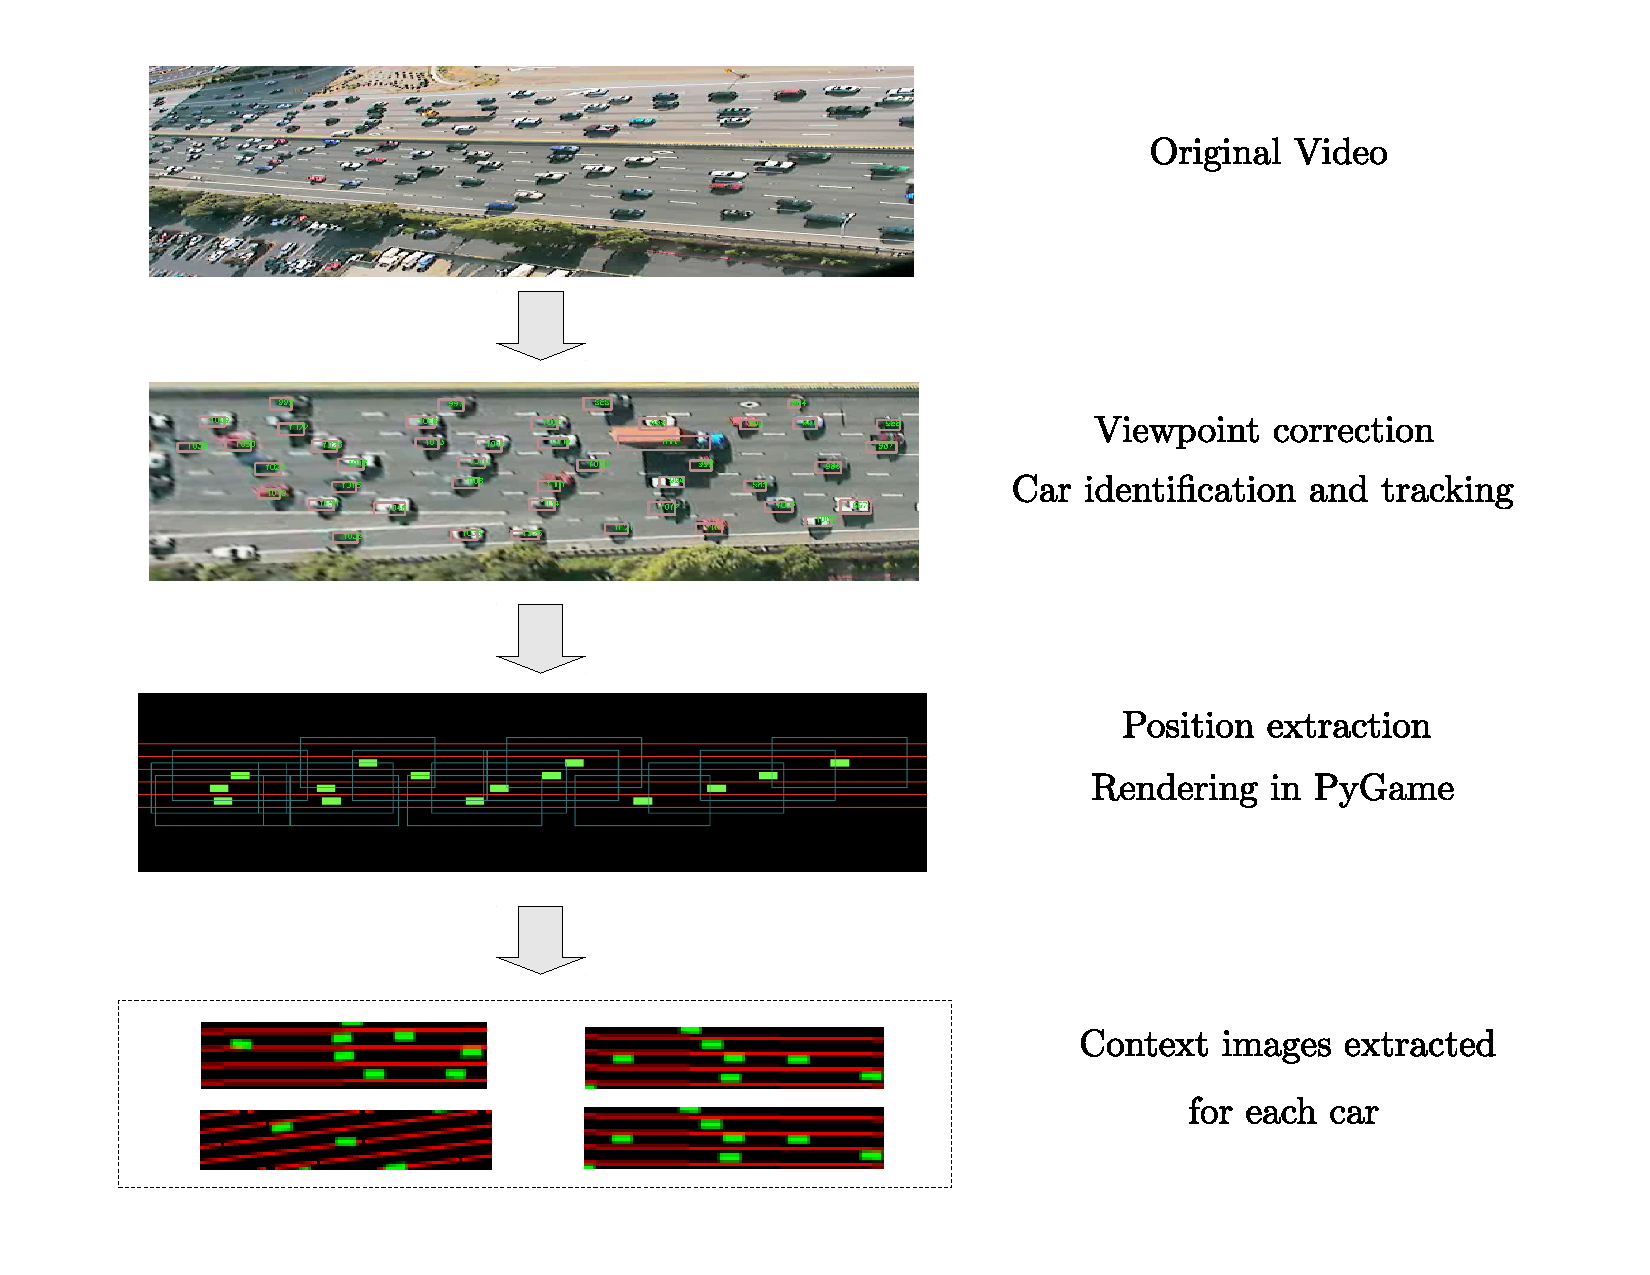
\includegraphics[width=\textwidth]{images/i80_preprocess.pdf}
  \end{subfigure}
  \caption{Preprocessing pipeline for the NGSIM-I80 data set.}
\end{figure}

\begin{figure}
  \centering
  \begin{subfigure}[b]{0.5\textwidth}
    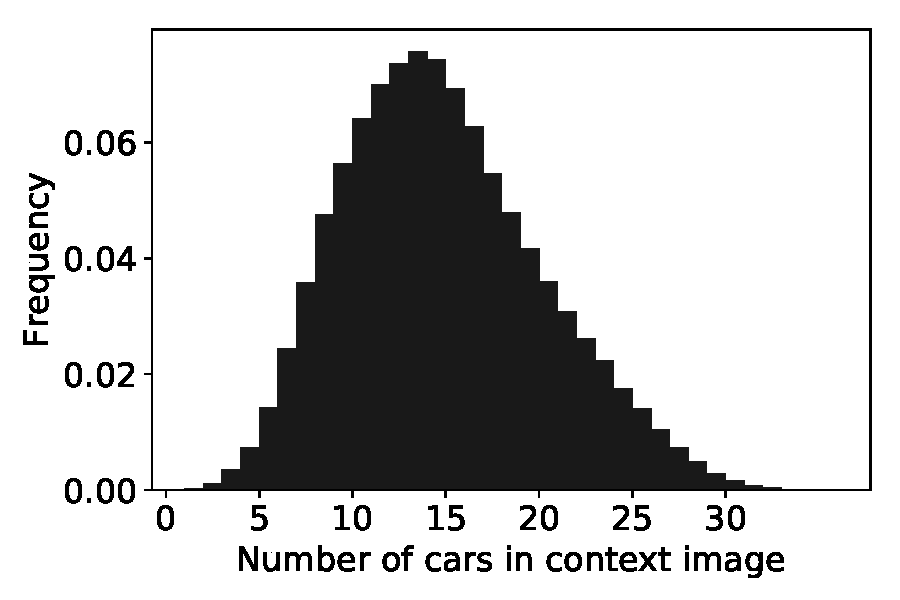
\includegraphics[width=\textwidth]{images/car_statistics.pdf}
  \end{subfigure}
  \caption{Cars per context state}
  \label{car-statistics}
\end{figure}

%We trained our latent variable forward model on a synthetic data set first --- where we are in partial control of the stochasticity of the data --- and on real vehicle trajectories afterwards.


\subsection{NGSIM I-80 freeway data set}

% \begin{figure}
%   \centering
%   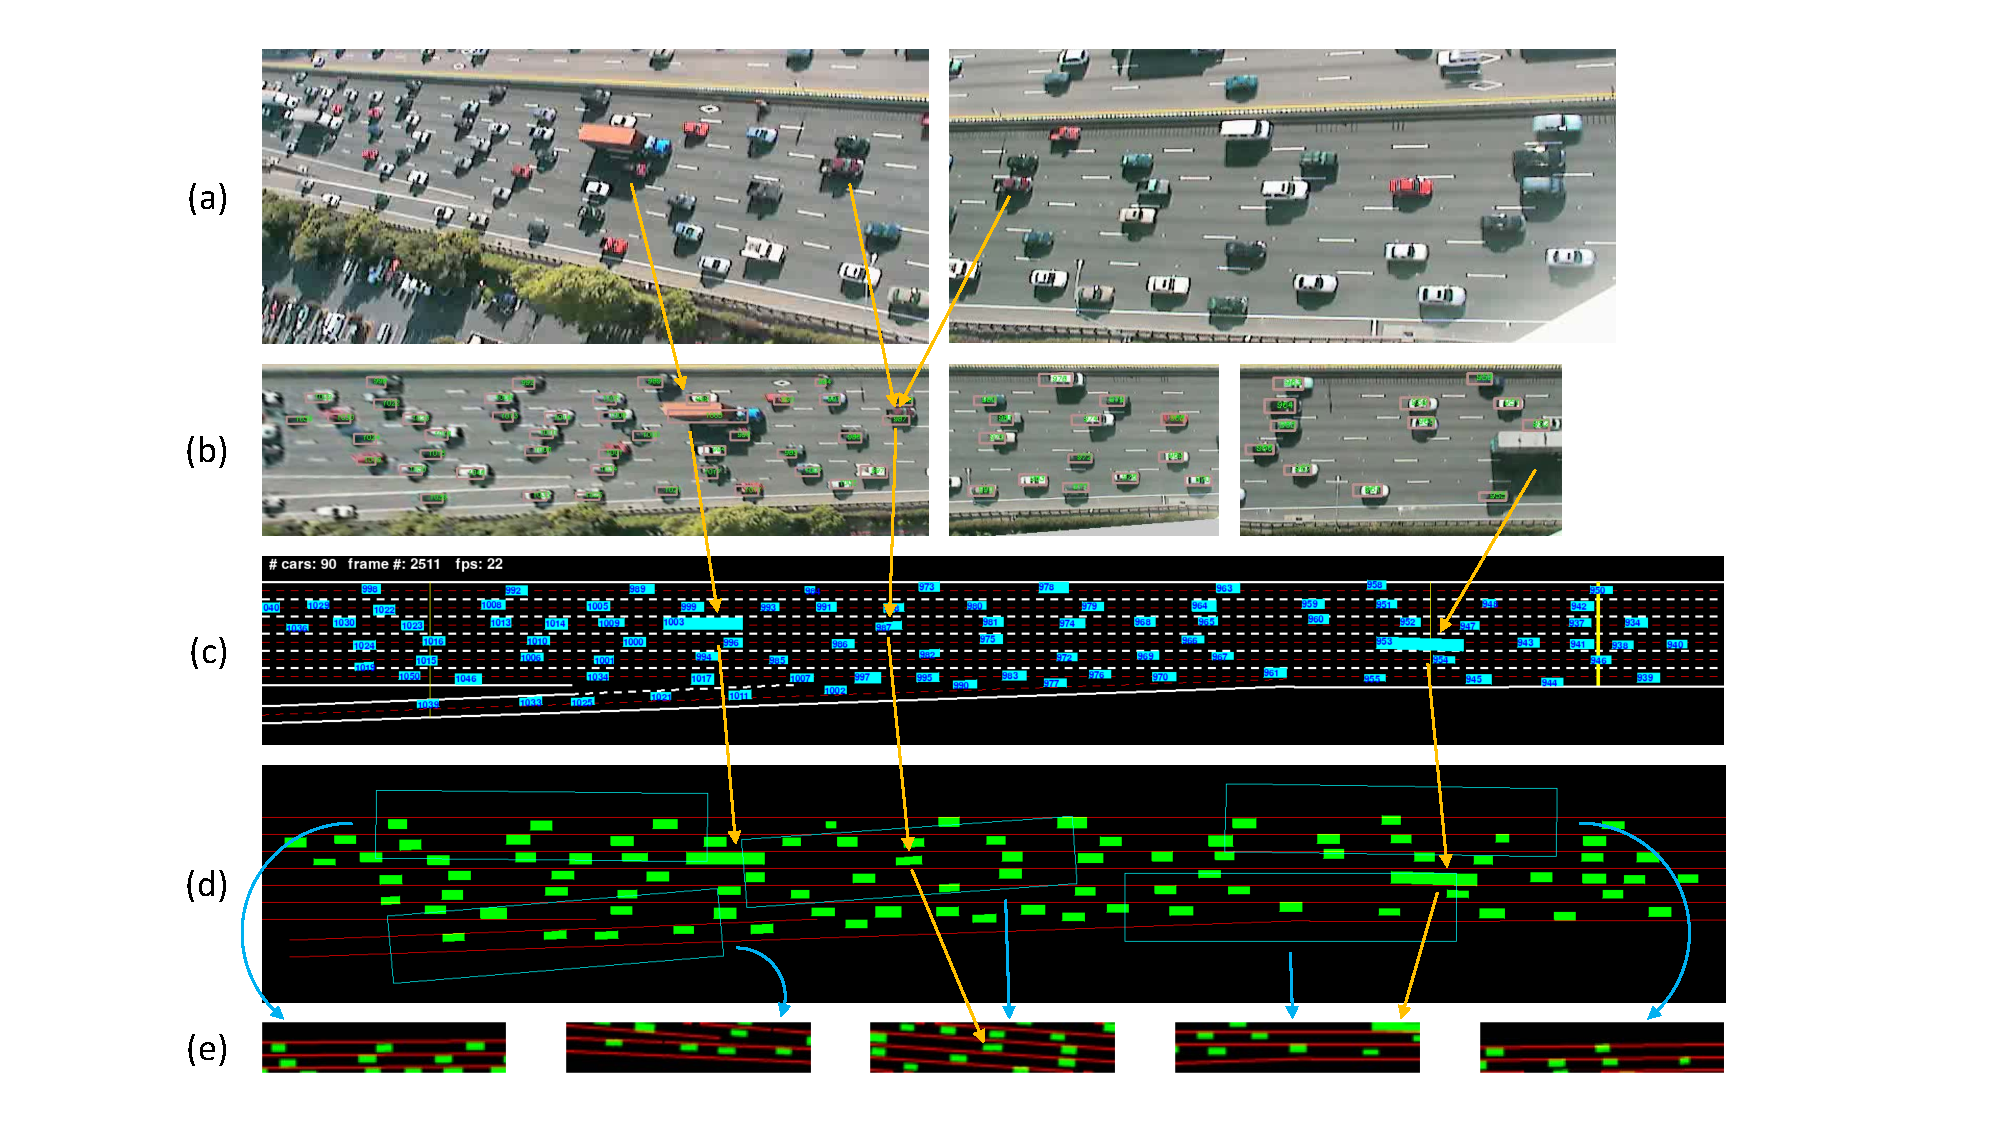
\includegraphics[width=4cm]{figures/I-80.png}
%   \caption{I-80 section schematic.}
% \end{figure}


\section{Experiments}

We evaluate our prediction model using two quantitative metrics in addition to visual evaluation.
\begin{itemize}
\item We follow the protocol used in previous works on stochastic generation \citep{Walker2016, Babaeizadeh2018, Denton2018}, where we generate a fixed number of samples using the stochastic model, compare each sample to the ground truth sample in the test set, and report the error of the best match.
  This method provides some measure of how well the stochastic model covers the space of possible futures, although it does not necessarily reflect the realism of all the generated samples.
\end{itemize}


\subsection{A note on evaluation}

We provide a discussion of evaluation metrics, and their relationship to the stochasticity of the prediction task.
Here we argue that the metric used in previous work \citep{Walker2016, Babaeizadeh2018, Denton2018} is only meaningful when the number of samples generated is of similar magnitude to the number of possible futures.
Consider the task of modeling a distribution of one-hot vectors, where each sample is a binary vector with all zeros except for a single $1$, whose index is chosen uniformly between $1$ and $n$.
A baseline model which always predicts the average $\tilde{y} = (1/n, 1/n, ..., 1/n)$ (which is clearly not a valid sample in the target distribution) will have an expected loss of $\sqrt{(n-1)/n}$. A stochastic model which exactly captures the true distribution will have an expected loss of $\sqrt{2} \cdot F(k, k, (n-1)/n)$, where $F$ refers to the cumulative distribution function of a Binomial random variable with $p=(n-1)/n$ (proofs can be found in the Appendix).
Curves of both of these loss functions for different $n$ are shown in Figure \ref{expected-loss}.
These illustrate that as $n$ becomes large, an increasingly high number of samples is required for the correct stochastic prediction model to outperform the deterministic baseline according to this metric.

The number of possible futures of a stochastic process can grow exponentially with the number of time steps.
We therefore use this metric to evaluate model predictions over a limited time horizon in order to give models a chance to capture the true future with a number of samples which is computationally tractable.
Since we are also interested in the the performance of models to generate predictions over long time horizons, we also provide a complementary measure where we train an separate model to distinguish between real and generated images after the stochastic model has been trained. This has been used in several works to evaluate GANs \citep{Danihelka17, Rosca17, GANeval}, however the approach is applicable to generative models more broadly. In this work we use the Least-Squares GAN Criterion \citep{Mao16}, as this was found to be both stable and sensitive in \citep{GANeval}.




\begin{itemize}
\item Gradient of $z$ vectors for single timestep
\end{itemize}



\begin{figure}
  \centering
  \begin{subfigure}[b]{0.45\textwidth}
    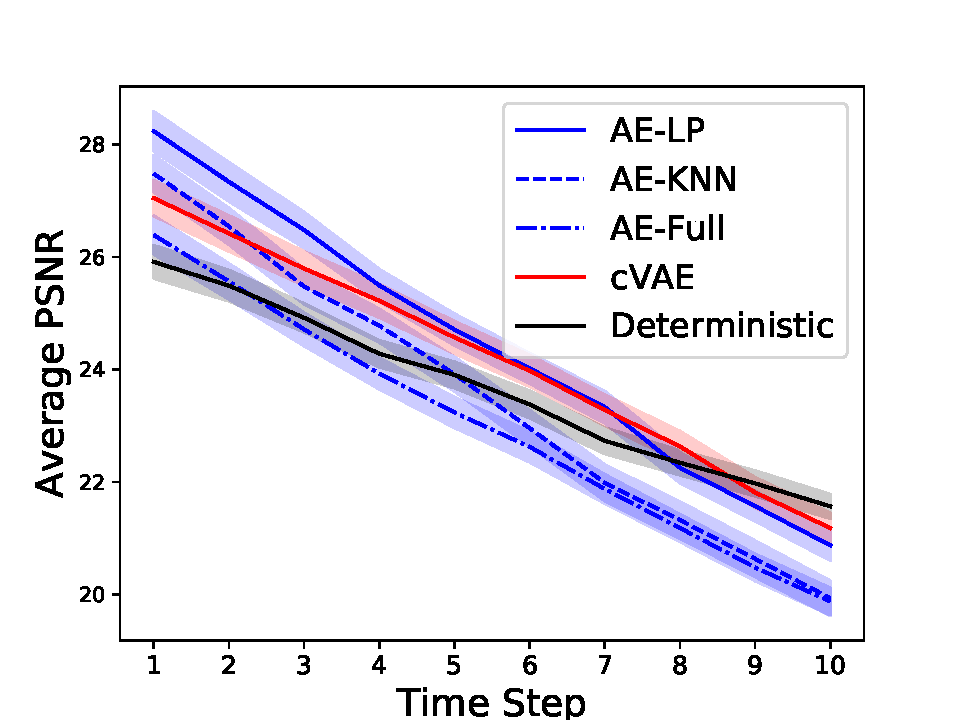
\includegraphics[width=\textwidth]{images/best_of_k_i80.pdf}
    \caption{A gull}
    \label{fig:gull}
  \end{subfigure}
  ~ %add desired spacing between images, e. g. ~, \quad, \qquad, \hfill etc.
  %(or a blank line to force the subfigure onto a new line)
  \begin{subfigure}[b]{0.45\textwidth}
    \includegraphics[width=\textwidth]{images/z_gradient-crop.pdf}
    \caption{A tiger}
    \label{fig:tiger}
  \end{subfigure}
  ~ %add desired spacing between images, e. g. ~, \quad, \qquad, \hfill etc.
  %(or a blank line to force the subfigure onto a new line)
  \caption{Pictures of animals}\label{fig:animals}
  \end{figure}










\begin{figure}
  \centering
  \begin{subfigure}[b]{0.4\textwidth}
    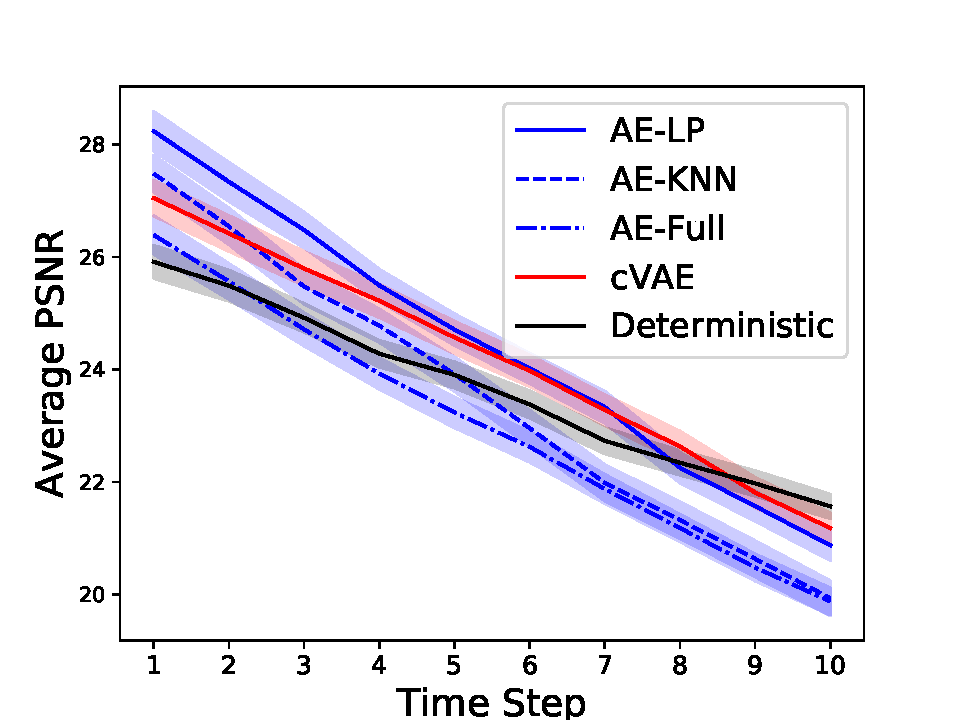
\includegraphics[width=\textwidth]{images/best_of_k_i80.pdf}
    \caption{Best-of-$k$ measure}
    \label{fig:gull}
  \end{subfigure}
  ~ %add desired spacing between images, e. g. ~, \quad, \qquad, \hfill etc.
  %(or a blank line to force the subfigure onto a new line)
  \begin{subfigure}[b]{0.25\textwidth}
  \centering
  \begin{tabular}{l|l|lll}
    \toprule
    Steps     & Det & cVAE & AE-LP & $p$-value \\
    \midrule
    500 & 0.00951 & 0.10296 & 0.11437 & 0.2134 \\
    1000 & 0.00183 & 0.00989 & \textbf{0.02681} & 0.0284 \\
    1500 & 0.00095 & 0.00168 & \textbf{0.00391} & 0.0068 \\
    2000 & 0.00059 & 0.00074 & \textbf{0.00154} & 0.0002 \\
    \bottomrule
  \end{tabular}
      \caption{Independent Critic Scores}
    \label{fig:tiger}
  \end{subfigure}
  ~ %add desired spacing between images, e. g. ~, \quad, \qquad, \hfill etc.
  %(or a blank line to force the subfigure onto a new line)
      \caption{Scores assigned by a critic independently trained to classify real samples from samples generated by the different models on the NGSIM-I80 dataset, averaged over 20 random seeds. $p$-value indicates whether the difference between cVAE and AE-LP scores is statistically significant according to a Wilcoxon rank-sum test.}

  \end{figure}









\subsection{Bair Robot Pushing Dataset}

To test the generality of our video prediction model, we also evaluated it on two other video prediction data sets used in the literature: Stochastic Moving MNIST introduced in \citep{Denton2018} and the BAIR robot pushing data set originally introduced in \citep{Ebert17} and used for video prediction in \citep{Babaeizadeh2018, Denton2018}.
We used the same model architectures as in \citep{Denton2018}: for BAIR, a VGG16 frame encoder and decoder combined with a 2-layer LSTM network with 128 hidden units, and for SM-MNIST a DCGAN encoder and decoder also combined with a 2-layer LSTM with 128 hidden units. All models were training with Adam \citep{ADAM} with learning rate $0.002$.
The main difference is that we did not use a prior network at training time, did not include a KL term in the loss function, and instead sampled latents at test time using the approaches described in Section 2.
We also set the dimension of $z$ to be lower (2 dimensions) and trained the model with dropout parameter $p=1$ on the latent code (corresponding to purely deterministic mode) until the loss stopped decreasing, after which we set $p=0.5$.

Results for our method and two other state-of-the-art methods using the best-of-$k$ metric are shown in Figure \ref{bair}. Our AE-LP variant performs best for the first few predicted timesteps according to both SSIM and PSNR. For predictions further into the future, the performance of AE-LP, AE-KNN and SVG-LP becomes statistically equivalent.  Interestingly, the relative performance of \citep{Babaeizadeh2018} depends on the performance metric. Examples of video generations can be found at \url{url}. We found that the AE-KNN variant was relatively robust to the choice of the hyperparameter $k$, a comparison of different settings as well as the full graph variant can be found in the Appendix. Overall, these results suggest that our architecture and non-parametric sampling approach are at least comparable to variational approaches. The fact that our model is able to achieve good performance using a latent variable of such small size (2 dimensions) also shows that this data set is in fact quite simple.

\begin{figure}
  \centering
  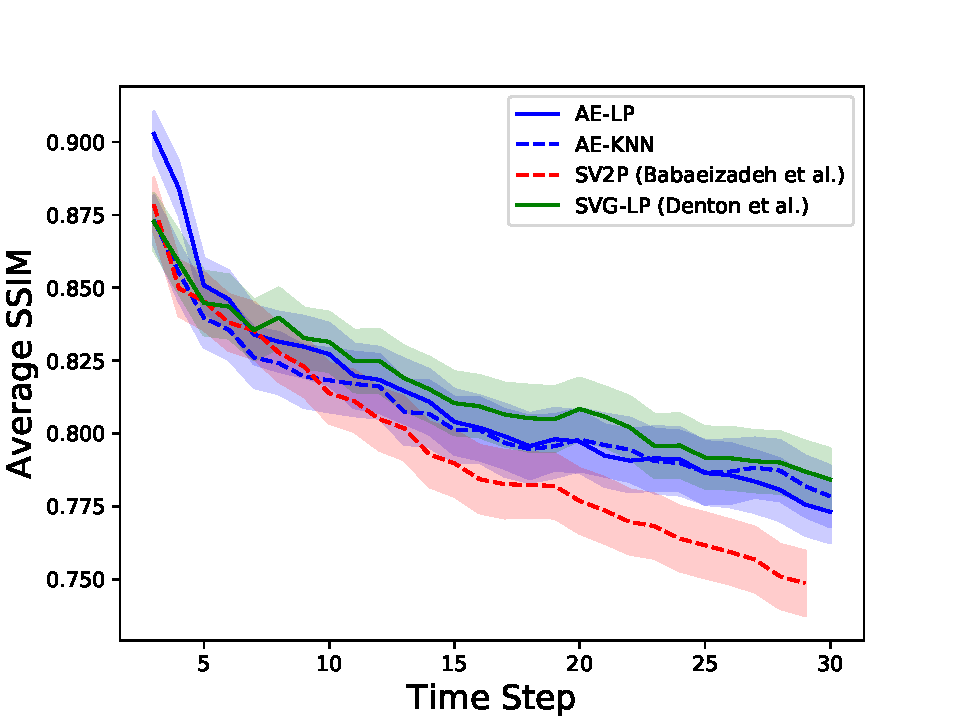
\includegraphics[width=0.4\textwidth]{images/bair_ssim.pdf}
  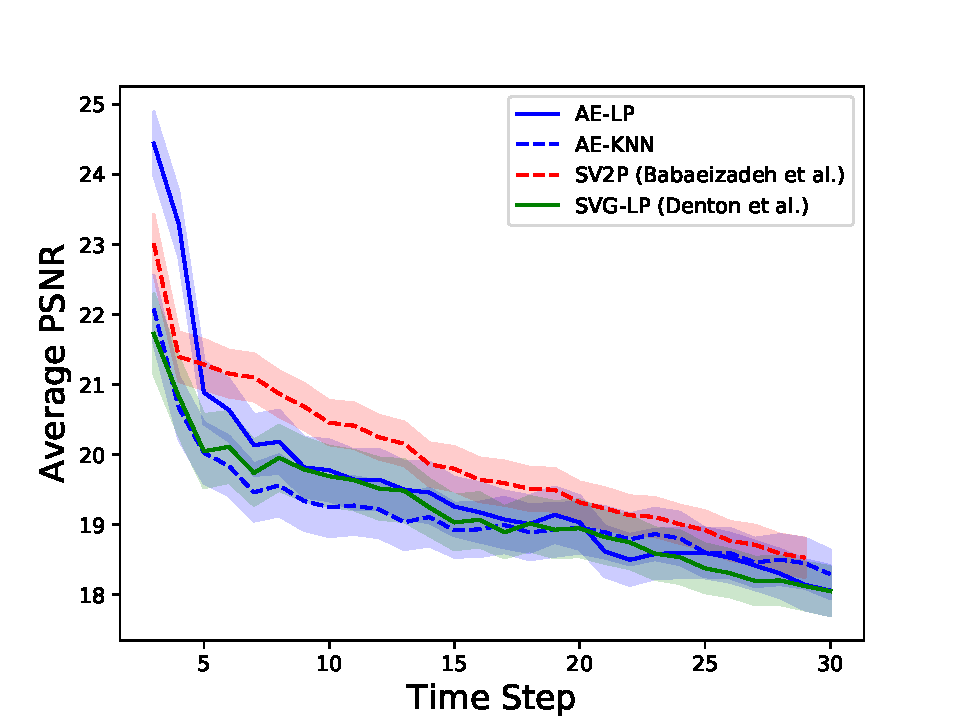
\includegraphics[width=0.4\textwidth]{images/bair_psnr.pdf}
%  \fbox{\rule[-.5cm]{0cm}{4cm}
%    \rule[-.5cm]{4cm}{0cm}}
  \caption{Best-of-$k$ performance on the BAIR data set, where the best PSNR and SSIM out of 200 generated samples compared to the test sample is reported. Shading indicates $95\%$ confidence interval. }
  \label{bair}
\end{figure}


\subsection{NGSIM-80 Driving Dataset}




\begin{figure}
  \centering
  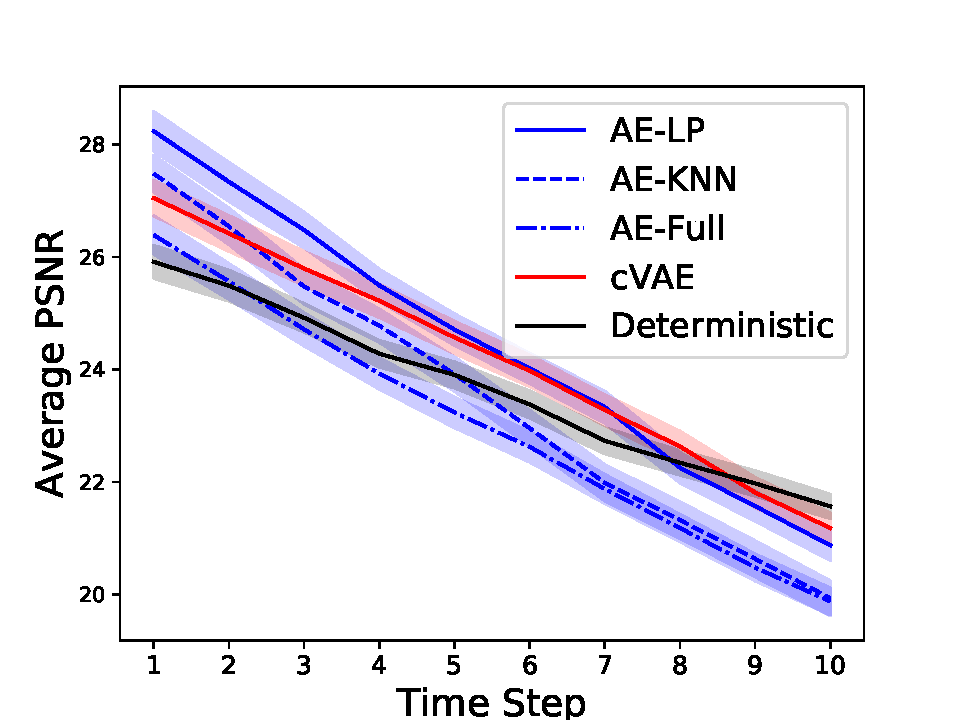
\includegraphics[width=0.5\textwidth]{images/best_of_k_i80.pdf}
%  \fbox{\rule[-.5cm]{0cm}{4cm}
%    \rule[-.5cm]{4cm}{0cm}}
  \caption{Best-of-$k$ performance on the NGSIM-I80 data set, where the best PSNR out of 200 generated samples compared to the test sample is reported. Shading indicates $95\%$ confidence interval. }
  \label{bair}
\end{figure}



\begin{table}
  \caption{Scores assigned by a critic independently trained to classify real samples from samples generated by the different models on the NGSIM-I80 dataset, averaged over 20 random seeds. $p$-value indicates whether the difference between cVAE and AE-LP scores is statistically significant according to a Wilcoxon rank-sum test.}
  \label{sample-table}
  \centering
  \begin{tabular}{l|l|lll}
    \toprule
    Training iteration     & Deterministic & cVAE & AE-LP & $p$-value \\
    \midrule
    500 & 0.00951 & 0.10296 & 0.11437 & 0.2134 \\
    1000 & 0.00183 & 0.00989 & \textbf{0.02681} & 0.0284 \\
    1500 & 0.00095 & 0.00168 & \textbf{0.00391} & 0.0068 \\
    2000 & 0.00059 & 0.00074 & \textbf{0.00154} & 0.0002 \\
    \bottomrule
  \end{tabular}
\end{table}


\begin{table}
  \caption{Timing for NGSIM-I80 data set}
  \label{sample-table}
  \centering
  \begin{tabular}{lll}
    \toprule
    Operation     & Time (s) \\
    \midrule
    Encoding & 0.0014  \\
    Decoding     & 0.0024 \\
    NN search over 100K codes & 0.0005      \\
    \bottomrule
  \end{tabular}
\end{table}



%\subsection{Figures}
%
%
%
%\subsection{Tables}
%
%
%\begin{table}
%  \caption{Sample table title}
%  \label{sample-table}
%  \centering
%  \begin{tabular}{lll}
%    \toprule
%    \multicolumn{2}{c}{Part}                   \\
%    \cmidrule(r){1-2}
%    Name     & Description     & Size ($\mu$m) \\
%    \midrule
%    Dendrite & Input terminal  & $\sim$100     \\
%    Axon     & Output terminal & $\sim$10      \\
%    Soma     & Cell body       & up to $10^6$  \\
%    \bottomrule
%  \end{tabular}
%\end{table}
%
%\section{Final instructions}


\section{Appendix}







\subsection{Proof of Expected Loss}

The baseline model always produces the same prediction $\tilde{y} = (\frac{1}{n}, ..., \frac{1}{n})$. Each sample from the true distribution is of the form $y_i = (0, ..., 0, 1, 0, ..., 0)$ with a single non-zero element.
\begin{align}
  \mathbb{E}[\mathcal{L}_{\mbox{baseline}}] &= \sqrt{\sum_{i=1}^n (\tilde{y}_i - y_i)^2} \\
  &= \sqrt{(1-\frac{1}{n})^2 + (n-1)\Big ( \frac{1}{n} \Big )^2} \\
  &= \sqrt{\frac{(n-1)^2 + (n-1)}{n^2}} \\
  &= \sqrt{\frac{n-1}{n}}
\end{align}

To compute the best-of-$k$ loss, the true stochastic model produces $k$ samples of the same form as the one drawn from the true distribution, i.e. $\tilde{y}_k = (0, ..., 0, 1, 0, ..., 0)$, where the non-zero index is chosen uniformly from $1$ to $n$.
Let $j$ denote the non-zero index of the sample drawn from the true distribution and $i_1, i_2, ..., i_k$ non-zero indices of the samples output by the stochastic model.
The probability of each sample \textit{not} matching $y_j$ is equal to $p=\frac{n-1}{n}$.
Therefore, the probability of none of the generated samples matching $y_j$ is equal to the cumulative distribution function of a binomial random variable $B(k, p)$, denoted $F(k, k, p)$.
In the case of a generated sample matching $y_j$, the best-of-$k$ loss will equal 0, otherwise it will equal $\sqrt{2}$.

Putting this together, the expected best-of-$k$ loss is given by:

\begin{align}
  \mathbb{E}[\mathcal{L}_{\mbox{best-of-$k$}}] &= \mbox{P(at least one sample matches)}\cdot 0 + \mbox{P(none of the samples match)} \cdot \sqrt{2} \\
  &= \sqrt{2} \cdot F\Big (k, k, \frac{n-1}{n} \Big) \\
\end{align}


\begin{figure}
  \centering
  \begin{subfigure}[b]{0.3\textwidth}
    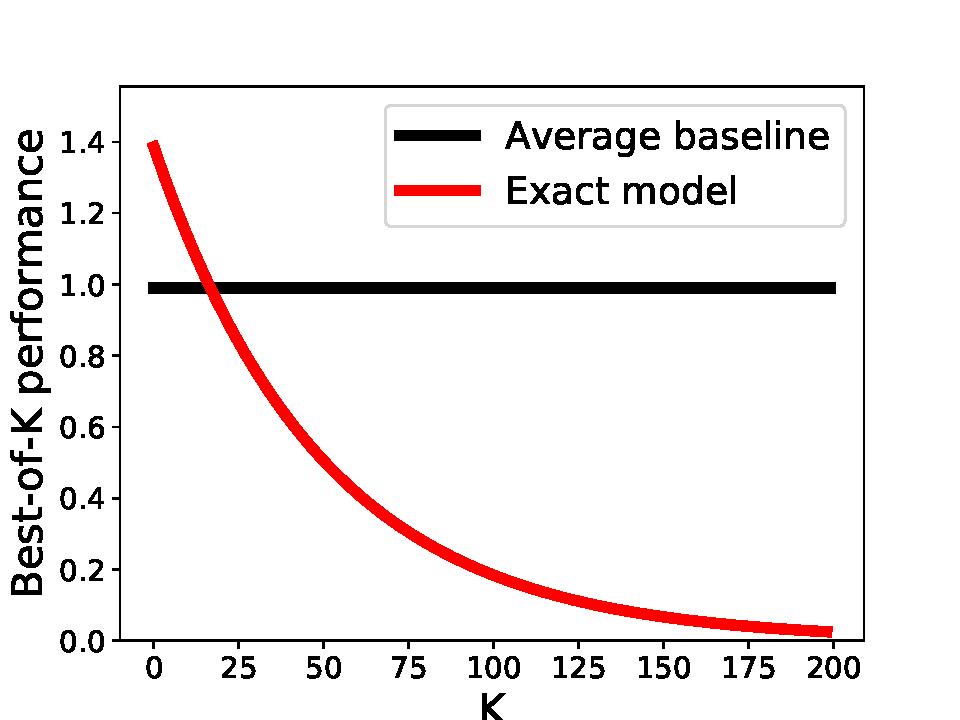
\includegraphics[width=\textwidth]{images/best_of_k_toy_n50.pdf}
    \caption{$n=50$}
    \label{fig:gull}
  \end{subfigure}
  ~ %add desired spacing between images, e. g. ~, \quad, \qquad, \hfill etc.
  %(or a blank line to force the subfigure onto a new line)
  \begin{subfigure}[b]{0.3\textwidth}
    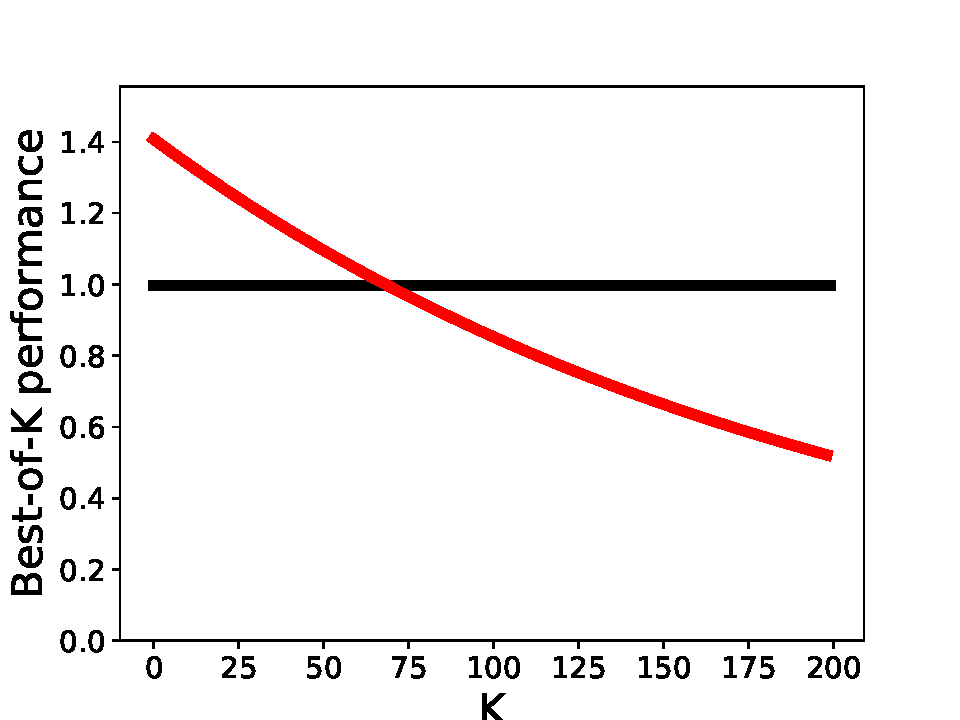
\includegraphics[width=\textwidth]{images/best_of_k_toy_n200.pdf}
    \caption{$n=200$}
    \label{fig:tiger}
  \end{subfigure}
  ~ %add desired spacing between images, e. g. ~, \quad, \qquad, \hfill etc.
  %(or a blank line to force the subfigure onto a new line)
  \begin{subfigure}[b]{0.3\textwidth}
    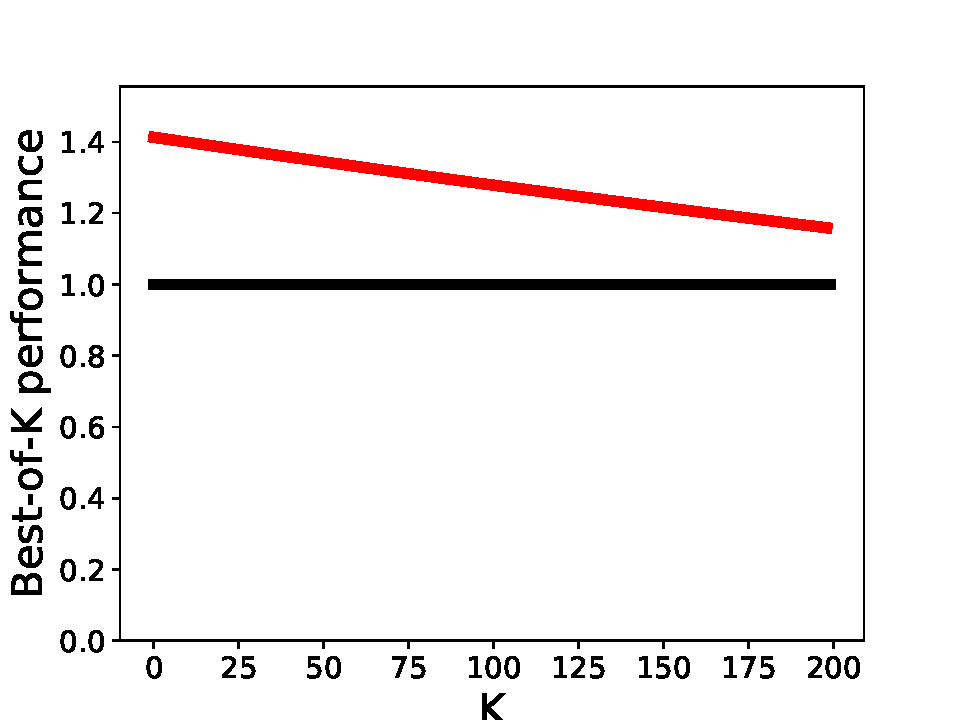
\includegraphics[width=\textwidth]{images/best_of_k_toy_n1000.pdf}
    \caption{$n=1000$}
    \label{fig:mouse}
  \end{subfigure}
  \caption{Best-of-$k$ performance of average baseline model and true model for different numbers of possible futures $n$. As the number of futures increases, it becomes increasingly difficult for the true model to outperform the baseline according to this metric.}\label{expected-loss}
  \end{figure}




\subsection{Additional Video Prediction Results}

\begin{figure}
  \centering
  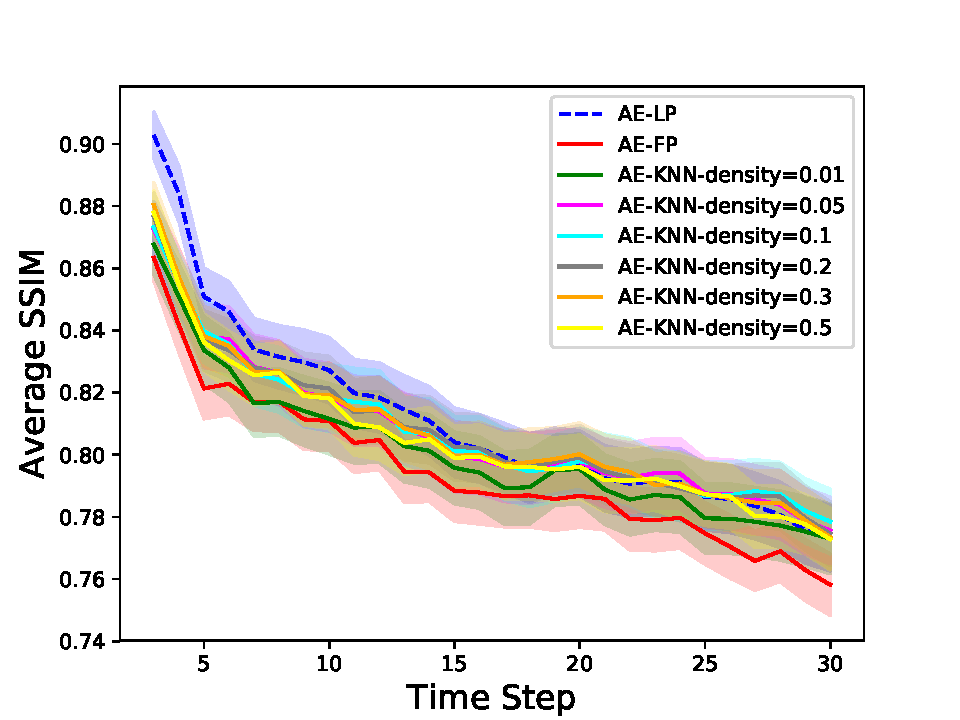
\includegraphics[width=0.4\textwidth]{images/bair_ae_comparison_ssim.pdf}
  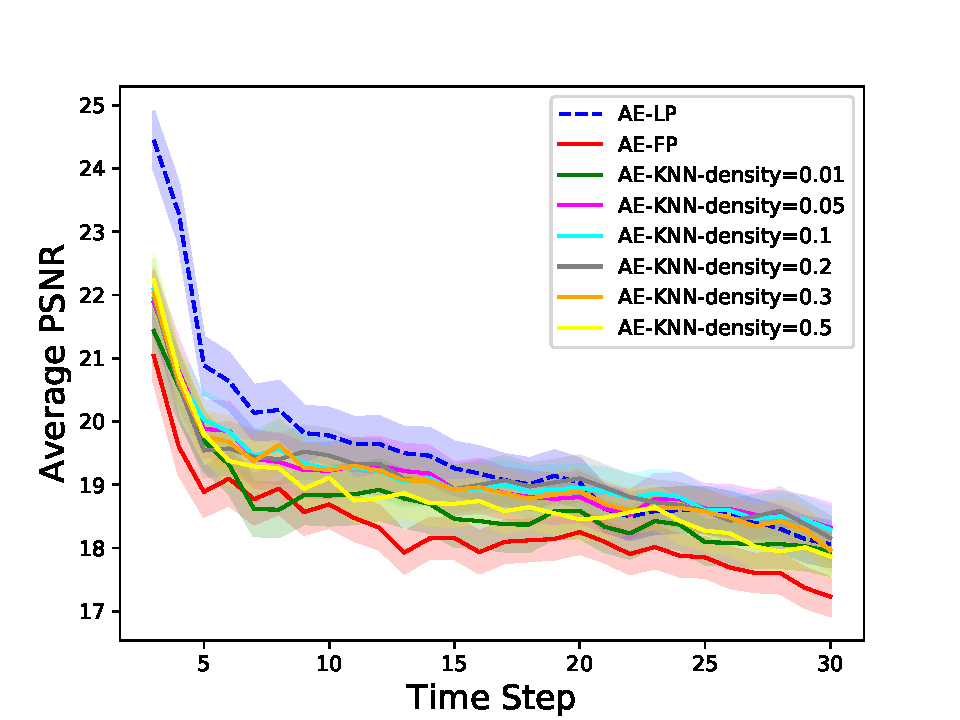
\includegraphics[width=0.4\textwidth]{images/bair_ae_comparison_psnr.pdf}
  \caption{}
  \label{bair}
\end{figure}


\begin{figure}
  \centering
  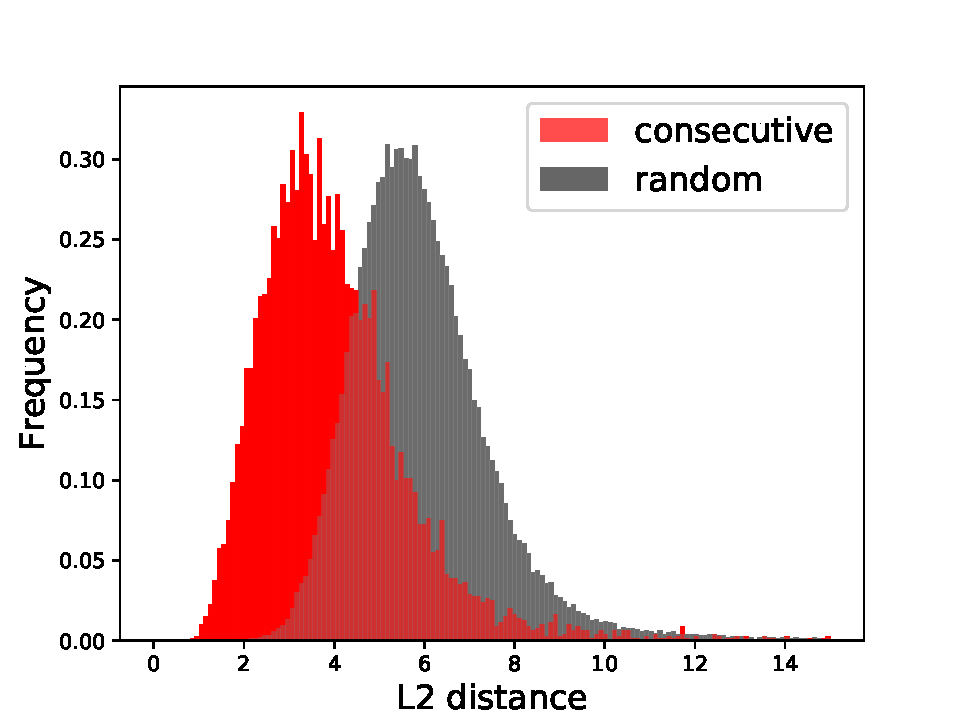
\includegraphics[width=0.5\textwidth]{images/distance_histograms.pdf}
%  \fbox{\rule[-.5cm]{0cm}{4cm}
%    \rule[-.5cm]{4cm}{0cm}}
  \caption{Distribution of distances between consecutive $z$ and random pairs of $z$ vectors extracted from the I-80 training set. Consecutive vectors are closer on average, which supports the smoothness assumption underlying Algorithm \ref{knn-algo}.}
\end{figure}



% \subsubsection*{Acknowledgments}
%
% Use unnumbered third level headings for the acknowledgments. All
% acknowledgments go at the end of the paper. Do not include
% acknowledgments in the anonymized submission, only in the final paper.

\bibliographystyle{unsrt}
\bibliography{nips_2018}

% \section*{References}
%
% References follow the acknowledgments. Use unnumbered first-level
% heading for the references. Any choice of citation style is acceptable
% as long as you are consistent. It is permissible to reduce the font
% size to \verb+small+ (9 point) when listing the references. {\bf
%   Remember that you can use more than eight pages as long as the
%   additional pages contain \emph{only} cited references.}
% \medskip
%
% \small


\end{document}
